\documentclass[a4paper, 11pt]{article}

\usepackage{caption}
\DeclareCaptionLabelFormat{adja-page}{\hrulefill\\#1 #2 {(see previous page)}}

\usepackage{graphicx}
\usepackage[export]{adjustbox}
\usepackage[left=1in,right=1in,top=1in,bottom=1in]{geometry}
\usepackage{xcolor}
\usepackage[bookmarksopen=true,pdfauthor=Lubos Polerecky,pdftitle=Look@NanoSIMS,pdfsubject=User manual]{hyperref}
\hypersetup{colorlinks=true,linkcolor=blue,urlcolor=blue}
\linespread{1.2}

\title{{\LARGE \bf Look@NanoSIMS}\footnote{\textbf{Citation}: L. Polerecky et al. (2012). Look@NanoSIMS --- a tool for the analysis of nanoSIMS data in environmental microbiology. \textit{Environmental Microbiology} 14 (4): 1009--1023. DOI: 10.1111/j.1462-2920.2011.02681.x}}
\author{{\large\bf Lubos Polerecky}\footnote{Feedback and questions can be sent to: l.polerecky@uu.nl}\\[6mm]
{\small Department of Earth Sciences, Utrecht University, Utrecht, The Netherlands (2013--today)} \\%[1mm]
{\small Max-Planck Institute for Marine Microbiology, Bremen, Germany (2002--2013)}\\[3mm]}
\date{User's manual, version 28-06-2025}

\definecolor{darkgold}{RGB}{120,75,4}
\definecolor{darkgreen}{RGB}{4,120,4}
\definecolor{purple}{RGB}{128,0,128}
\newcommand{\ttt}[1]{\texttt{#1}}
\newcommand{\lans}[1]{{\color{magenta}#1}}
\newcommand{\lanscb}[1]{{\color{darkgreen}#1}}
\newcommand{\lanstf}[1]{{\color{cyan}#1}}
%\newcommand{<name>}[<args>]{ <code> }
\usepackage{marginnote}
\newcommand\mnote{\marginnote{\fbox{\textbf{\bf Note}}}}
\newcommand\ra{\rightarrow}
\newcommand\addon[1]{-- {\small #1}}
\newcommand\figref[0]{\textbf{Figure}}
%\newcommand\s[1]{\noindent\textbf{Step #1:}}
\newcounter{step}
\setcounter{step}{0}
%\newcommand\s{\addtocounter{step}{1}\paragraph{Step \thestep:}\hspace{-2mm}}
\newcommand\s{\addtocounter{step}{1}\noindent\textbf{Step \thestep:}{ }}
\newcommand\bul{\noindent$\bullet${ }}
\newcommand\bb[1]{\textbf{#1}}

\begin{document}

\maketitle
\reversemarginpar 

%%

\section*{Summary}
\textbf{Look@NanoSIMS}, or shortly \textbf{LANS}, is a program for processing and analysis of ion count image data produced by the NanoSIMS instrument. The original development of the program started back in 2008, but its active development continues until today based on input and requests from users. Although the program may be considered an `old school' in a number of aspects, it has matured well over the years. Once you get used to it, become aware of all of its features and figure out all the tricks, it allows you to analyze NanoSIMS data very efficiently. This document describes how to get started with the program and carry out such analyses at a~basic, intermediate and advanced level. 

%%

\tableofcontents

\section{Installation instructions}

LANS is a Matlab-based program. Thus, a core \textbf{Matlab} installation, along with image processing and statistical toolboxes, is required to run LANS and perform basic functions. This makes it possible to run LANS on a variety of operating systems, including Linux, Microsoft Windows and MacOS. However, this also limits LANS to users with access to a Matlab license. Additionaly functionality of LANS is achieved by integrating the program with \textbf{\LaTeX} (for exporting results in a nicely formatted PDF output) and data compression programs such as \textbf{zip} (for decompressing input files and compressing output generated by LANS), both of which are available for free.

%%

\subsection{Install Matlab}

\begin{enumerate}

\item Matlab is available from \url{www.mathworks.com} and requires a license. It is useful to check whether your institution has a site-license (e.g., your university may have one for all students and academic staff). 

\item Version 2019b of Matlab is most recommended to ensure that all features of LANS work as designed. LANS works with newer Matlab versions as well, however, there is a risk that some functionality will issue errors due to less than perfect back-compatibility of Matlab.

\item When installing Matlab, you will need the \emph{core Matlab} and \emph{two toolboxes}: image processing and statistics and machine learning. 

\end{enumerate}

\mnote
Some output generated by LANS, e.g., information generated during the alignment of planes and stored in the file \ttt{xyalign.mat}, may not be read correctly by the Matlab version 2019b if it was generated by a newer Matlab version. Thus, if you plan to use LANS in collaboration with other people, e.g., by sharing the files generated by LANS among each other, it is recommended that everyone in the team uses the same Matlab version.

%%

\subsection{Install \LaTeX}

This software is required to enable export of graphical output as tagged PDF documents. 

\begin{enumerate}
 
\item To install \LaTeX, use one of the well-established \LaTeX\ distributions for your operating system, as described on the \href{https://www.latex-project.org/get/}{\LaTeX\ project} website (e.g., \ttt{texlive} for Linux, \ttt{MikTeX} for Windows, \ttt{MacTex} for MacOS). Note that the on-line LaTeX service, such as Overleaf, is insufficient; you really need a locally installed \LaTeX\ distribution.
 
\item To correctly integrate \LaTeX\ with LANS, you will need the following executables and packages installed and working:
 
\begin{itemize}
\item executables: \ttt{epstopdf}, \ttt{pdflatex}
\item packages: \ttt{graphicx}, \ttt{geometry}, \ttt{hyperref}, \ttt{adjustbox}
\end{itemize}
 
\end{enumerate}
 
\mnote
If you have never used \LaTeX\ on your computer, it may be that some \LaTeX\ packages, parti\-cu\-larly \ttt{geometry} and \ttt{hyperref}, are not installed during the 'standard' installation procedure. As a result, the execution of the LANS functions \lans{Export LaTeX and PDF output} (main LANS) or \lans{Export images for each variable as PDF} (Process metafile) may get stuck if the packages are missing. If this happens, you can fix this problem by compiling the \ttt{tex} file using the native \LaTeX\ environment (e.g., open the \ttt{tex} file in the default editor of your \LaTeX\ distribution and then compile it into a \ttt{pdf} output from there). When doing so, the missing \LaTeX\ packages should automatically be installed and the \ttt{tex} file should compile into a correct \ttt{pdf} output. Once this is done, the automatic \LaTeX\ compilation from within Matlab will also work.

%%

\subsection{Install software for compressing/decompressing files}

This software is required for two reasons.

\begin{enumerate}
 
\item It enables you to load compressed nanoSIMS datasets (\ttt{im.zip} files) by LANS. This is a useful feature because \ttt{im.zip} files have roughly a 10-fold smaller size than the original \ttt{im} files generated by the Cameca's nanoSIMS measurement software. It is recommended to store and distribute the raw data files by first compressing them with the \ttt{zip} program (extension \ttt{im.zip}). 

\item It allows you to compress the processed data generated by LANS. This is convenient for making data backups, since it is much more efficient to upload and download few compressed folders than hundreds of smaller files present in those folders.

\item \ttt{7-Zip} (freeware) is recommended for Microsoft Windows. \ttt{zip} and \ttt{unzip} are available by default on Linux and MacOS systems.

\end{enumerate}

%%

\subsection{Install Look@NanoSIMS}

This is done by simply copying the source files to a folder on your computer.

\begin{enumerate}
 
\item For convenience, the compressed file containing the \emph{latest version of LANS} is stored in this \href{https://www.dropbox.com/sh/gyss2uvv5ggu2vl/AABViAmt9WHryEP_xZBrCG_La?dl=0}{Dropbox folder}. Click on the \ttt{program} folder and then download the file \ttt{LANS-latest-src.zip}.

\item Unzip \ttt{LANS-latest-src.zip} to a folder of your choice.

\item Rename the \ttt{src} folder using a more reasonable name (e.g., \ttt{LANS-2025-05-26}, where the date will refer to the LANS version).

\end{enumerate}

\mnote
In case the Dropbox link above does not work, because it became outdated or the official distribution location changed, visit the LANS github repository or try to search the internet for more updated information. For users familiar with git and github, LANS can be downloaded by pulling the source code from the \ttt{src} folder in the LANS github repository: \url{https://github.com/lpolerecky/LANS}.

%%

\subsection{Starting Look@NanoSIMS for the first time}

Before you run LANS for the first time, revise the content of the files \ttt{lookatnanosims.m} and \ttt{lans\_paths.m}. These two files contain important settings you need to adjust to reflect your specific local installation of LANS. For example, you can specify there:

\begin{itemize}
\item locations of the compression/decompression software,
\item location of the PDF viewer,
\item default name of the file containing regions of interest (ROIs),
\item default extension of the raw data files.
\end{itemize}

\mnote
If you browse through the LANS installation files, you will notice that the \ttt{*.fig} files, which define the graphical user interface (GUI), appear in two sub-folders: \ttt{figs} and \ttt{figs\_win}. This is required because GUI defined on Unix-like and Windows platforms do not look the same. This is an issue due to --- apparently --- limited cross-platform compatibility of Matlab visual objects. However, this issue is not important for you as an end-user of LANS. You only need to be aware of it. Should you wish to modify any of the \ttt{*.fig} files, you will need to modify those that correspond to your operating system.

%%

\subsection{Starting Look@NanoSIMS on a regular basis}

\begin{enumerate}

\item Start Matlab.

\item Set the current folder to the folder where you installed LANS. You can do this through the menu or, more easily, entering one of the following commands in the Matlab console. The precise syntax depends on whether you use Windows, Linux or MacOS, and on the path where you installed LANS. Thus, you will need to adapt them according to your local settings.

\ttt{>> cd c:/programs/LANS}

\ttt{>> cd /home/your\_username/programs/LANS}

\item Once you are in the correct folder, enter the following command in the Matlab console:

\ttt{>> lookatnanosims}

If everything is set up correctly, the main LANS graphical user interface (GUI) will open, as shown in Fig.~\ref{fig1:mainLANSgui}. You can start from there, as described in the following sections of this document. 

\end{enumerate}

\begin{figure}[!t]
\centering
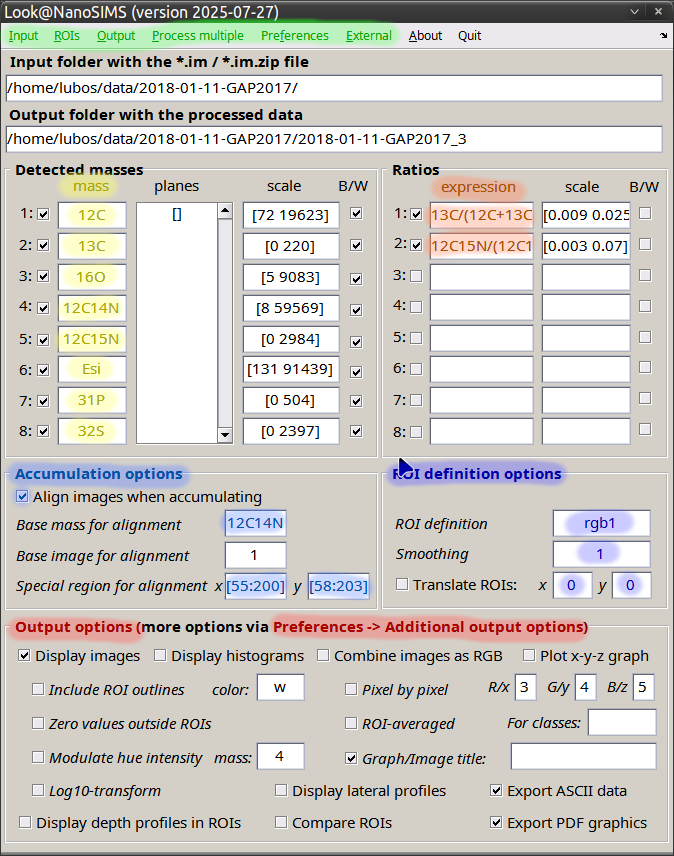
\includegraphics[width=0.9\textwidth]{figs1/LANS-maingui}
\caption{\label{fig1:mainLANSgui}%
Main graphical user interface (GUI) of Look@NanoSIMS.}
\end{figure}

\mnote
During the data processing session, LANS provides quite a lot of useful information in the Matlab console. Thus, it is a good idea to \emph{always} keep an eye on the output in the console. You can do this by arranging your desktop such that both the LANS and Matlab console windows are visible at the same time. This is also useful in case you encounter an error while working in LANS. These errors will be shown in the console, too.


%%

\subsection{Updating Look@NanoSIMS}

\begin{enumerate}
 
\item LANS is updated quite regularly. You can update it easily by entering in the Matlab console:

\ttt{>> lans\_webupdate} 

You need to be in the folder where LANS is installed to run this command. In the process, you will be prompted to make a backup of your older LANS version, which is recommended to do, just in case.

\item If you are familiar with \ttt{git}, you can update LANS by pulling the latest sources from the LANS github repository \url{https://github.com/lpolerecky/LANS}.

\end{enumerate}

%%%%

\section{Organization of the input and output data}
\label{sec:data_organization}

Working with LANS, and with nanoSIMS data in general, can be a book-keeping challenge. To start with, you will have many raw data files (\ttt{im} or \ttt{im.zip} files) acquired at different dates and from different types of samples (e.g., different treatments). Additionally, processing of those raw data files with LANS will create many output files, including ASCII data, PDF images, matlab output, PDF output, and zipped backed-up folders. It is therefore a good idea to develop and maintain a certain structure of those folders and output files, to \emph{keep everything organized}. 

In this document, we assume that the raw and processed nanoSIMS data are organized hierarchically as shown in Table~\ref{tab1:file_structure}. We have used this data organization at Utrecht University for many years, and it works pretty well. We therefore highly encourage users to adopt it as well. Its benefits will become more apparent later on, when we get to the point of explaining how to efficiently process and analyze \emph{multiple} nanoSIMS datasets from a particular project.

\begin{table}[hb]
\centering
\caption{\label{tab1:file_structure} Hierarchical organization of the raw and processed nanoSIMS data implemented in Look@NanoSIMS. An example of such data organization along with a more detailed explanation is shown in Figures~\ref{fig2:data_organizationAB} and~\ref{fig2:data_organizationCD}.}
\begin{tabular}{l@{ $\rightarrow$ }c@{ $\rightarrow$ }l@{ $\rightarrow$ }l@{ $\rightarrow$ }l}
\hline
root & project & measurment day 1 & raw dataset 1.1 & \color{red}{dataset folder} 1.1\\
\multicolumn{2}{c}{} & & raw dataset 1.2  & dataset folder 1.2\\
\multicolumn{2}{c}{} & & $\cdots$ & $\cdots$ \\
\multicolumn{1}{c}{} & & measurement day 2 & raw dataset 2.1  & dataset folder 2.1\\
\multicolumn{2}{c}{} & & raw dataset 2.2  & dataset folder 2.2\\
\multicolumn{2}{c}{} & & $\cdots$ & $\cdots$\\
\multicolumn{1}{c}{} & & $\cdots$ & $\cdots$ & $\cdots$\\
\hline
\multicolumn{2}{r}{\color{red}{dataset folder} $i$ $\rightarrow$} & \color{orange}{dat} & \multicolumn{2}{l}{\color{orange}{numbers}} \\
\multicolumn{2}{r}{$\rightarrow$} & \textcolor{darkgold}{pdf} & \multicolumn{2}{l}{\textcolor{darkgold}{images \&\ graphs}} \\
\multicolumn{2}{r}{$\rightarrow$} & \multicolumn{3}{l}{\hspace{-2mm}processing definition files (\textcolor{purple}{alignment, ROIs, preferences})} \\
\multicolumn{2}{r}{$\rightarrow$} & \multicolumn{3}{l}{\hspace{-2mm}\textcolor{purple}{OutputG.pdf (output summary)}}\\
\hline
\end{tabular}
\end{table}

At the highest level of the data organization is a root folder that contains \emph{all} nanoSIMS data. This folder contains `project folders' with nanoSIMS data belonging to \emph{specific projects}. Each `project folder' contains `day folders' with data acquired on \emph{different measurement days}. Each `day folder' contains the actual \emph{raw datasets} (\ttt{im} or \ttt{im.zip} files). When a particular raw dataset is processed and analyzed, the corresponding data is stored in a `dataset folder' with the \emph{same name} as the dataset. Each `dataset folder' contains sub-folders with the \emph{results} of the analysis, including numerical values such as ROI-specific ion counts or ion count ratios (folder \ttt{dat}), and graphical output such as images or scatter plots (folder \ttt{pdf}). The `dataset folder' also contains information defining the processing steps, such as alignment of frames, definition and classification of regions of interest (ROIs), and preferences. This information is useful if you want to go back to the analysis of the same dataset after you have analyzed a different one, e.g., to perform quality checks or more in-depth analyses. Finally, the `dataset folder' also contains a PDF file with a comprehensive graphical summary of the analysis. This file is useful if you wish to share the results for a specific dataset with project collaborators.


\begin{figure}[ht]
\centering
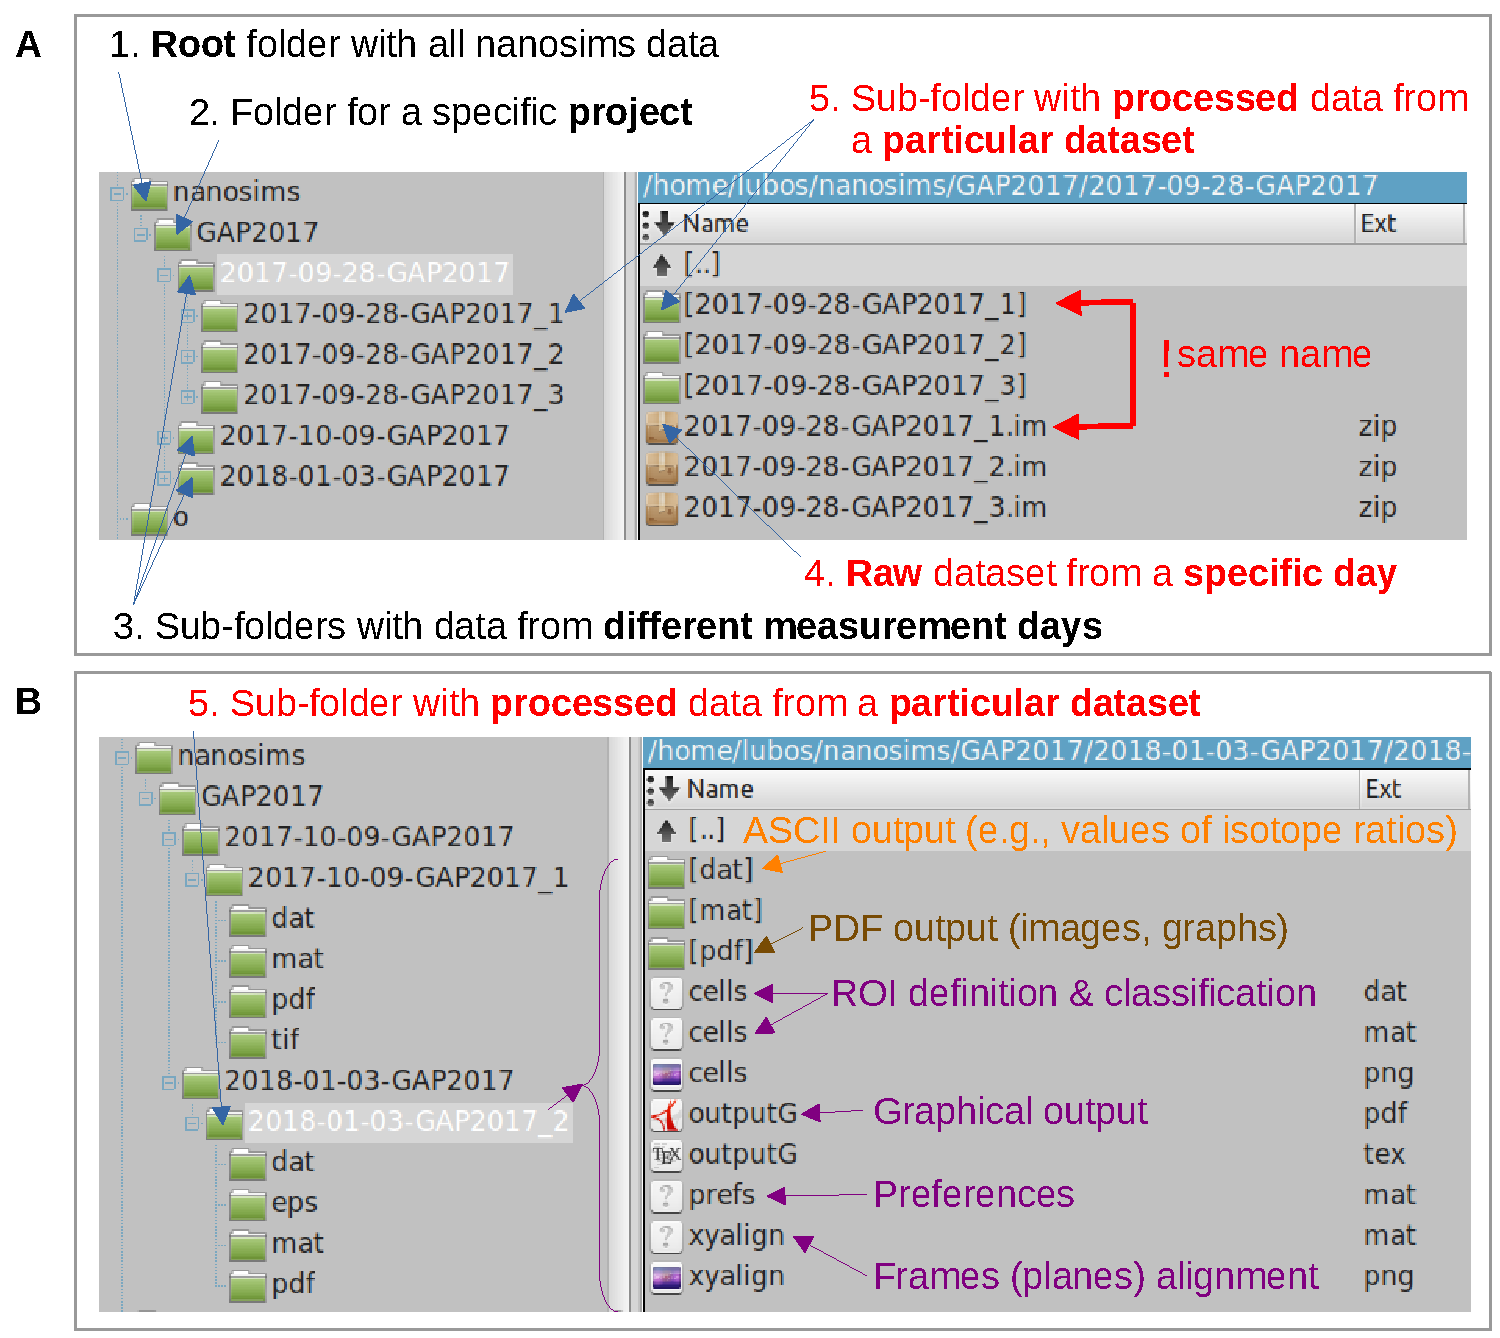
\includegraphics[width=\textwidth]{figs2/folders_organizationAB}
\caption{\label{fig2:data_organizationAB}%
	Example of a hierarchical organization of the raw and processed nanoSIMS data implemented in Look@NanoSIMS. %
  \textbf{(A)} The root folder (\ttt{nanosims}) contains a~project-specific sub-folder (e.g., \ttt{GAP2017}), which contains sub-folders with data measured on different days (e.g., \ttt{2017-09-28-GAP2017}, \ttt{2017-10-09-GAP2017}). %
  The `day folder' contains \emph{multiple raw datasets} measured on that particular day (\ttt{im} or \ttt{im.zip} files). %
  When a particular raw dataset is processed and analyzed, the data is stored in a `dataset folder' with the \emph{same name} as the dataset (see red ``!''). %
  \textbf{(B)} The `dataset folder' contains files defining the processing steps, including alignment information (\ttt{xyalign}), definition and classification of regions of interest (\ttt{cells.mat} and \ttt{cells.dat}, respectively), preferences (\ttt{prefs.mat}), and a comprehensive summary of results exported in a PDF file (\ttt{OutputG.pdf}). %
  See more information in Fig.~\ref{fig2:data_organizationCD}.%
}
\end{figure}
%\begin{figure} [t!]
%    \captionsetup{labelformat=adja-page}
%    \ContinuedFloat
%    \caption[Figure]{%

\begin{figure}[ht]
\centering
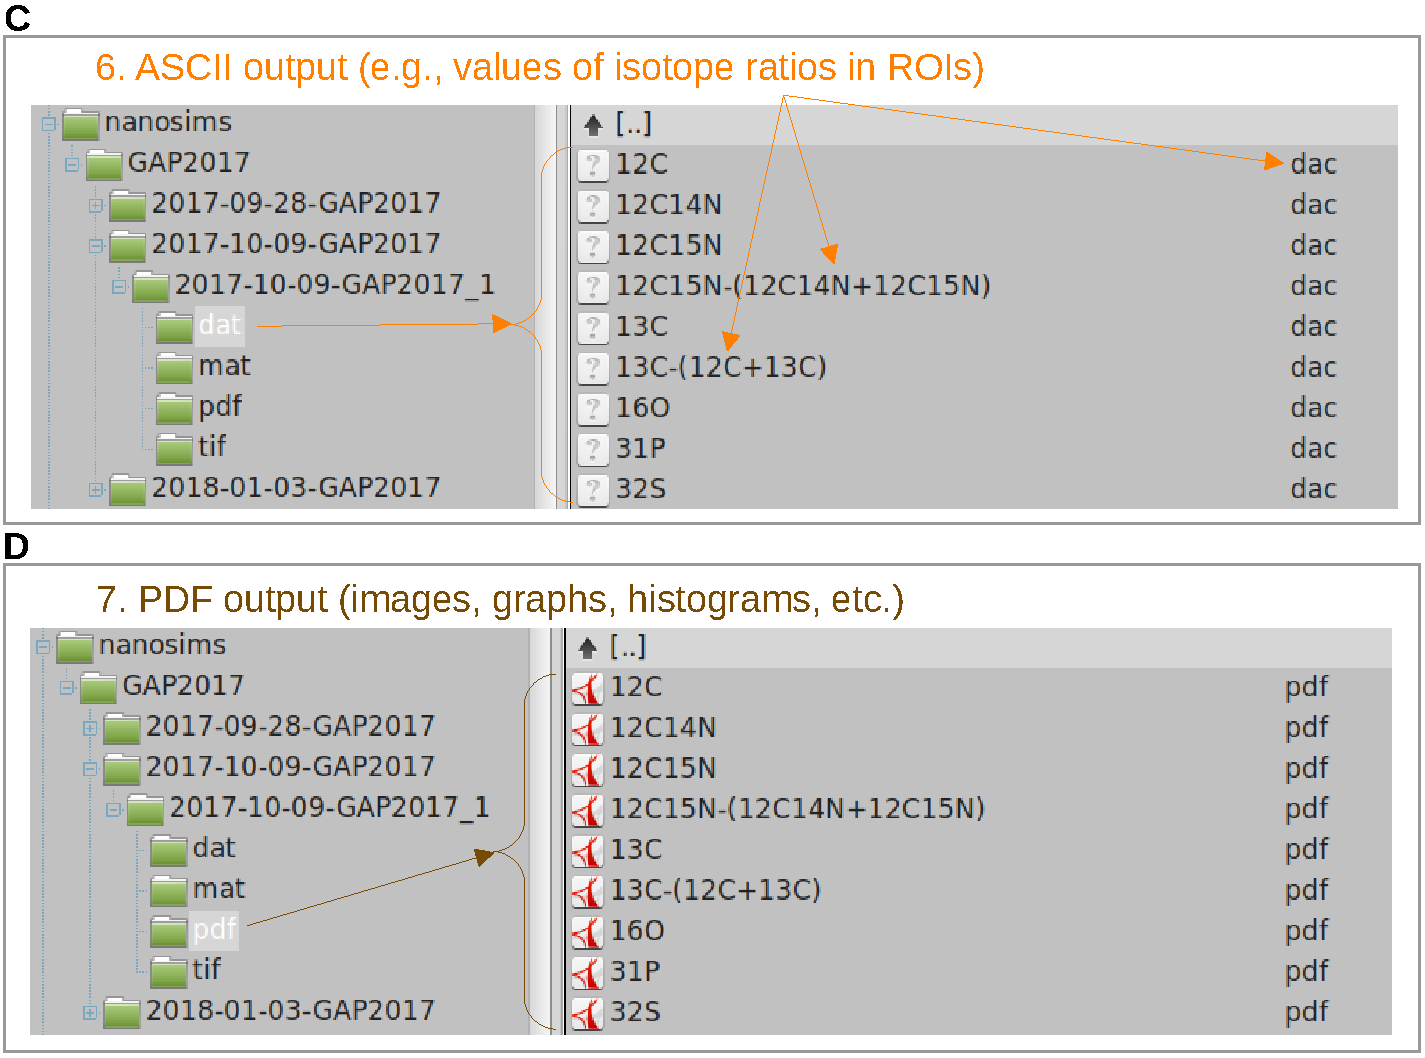
\includegraphics[width=\textwidth]{figs2/folders_organizationCD}
\caption{\label{fig2:data_organizationCD}%
  Continuation from Fig.~\ref{fig2:data_organizationAB}. %
The `dataset folder' also contains sub-folders with output generated by LANS in different formats. %
    \textbf{(C)} The ROI-specific ion counts and ion count ratios (\ttt{dac} files) are stored in the \ttt{dat} folder. %
    \textbf{(D)} The images, graphs, histograms, etc., are stored in the \ttt{pdf} folder.}
\end{figure}

%%

%\begin{figure}[b!]
%\centering
%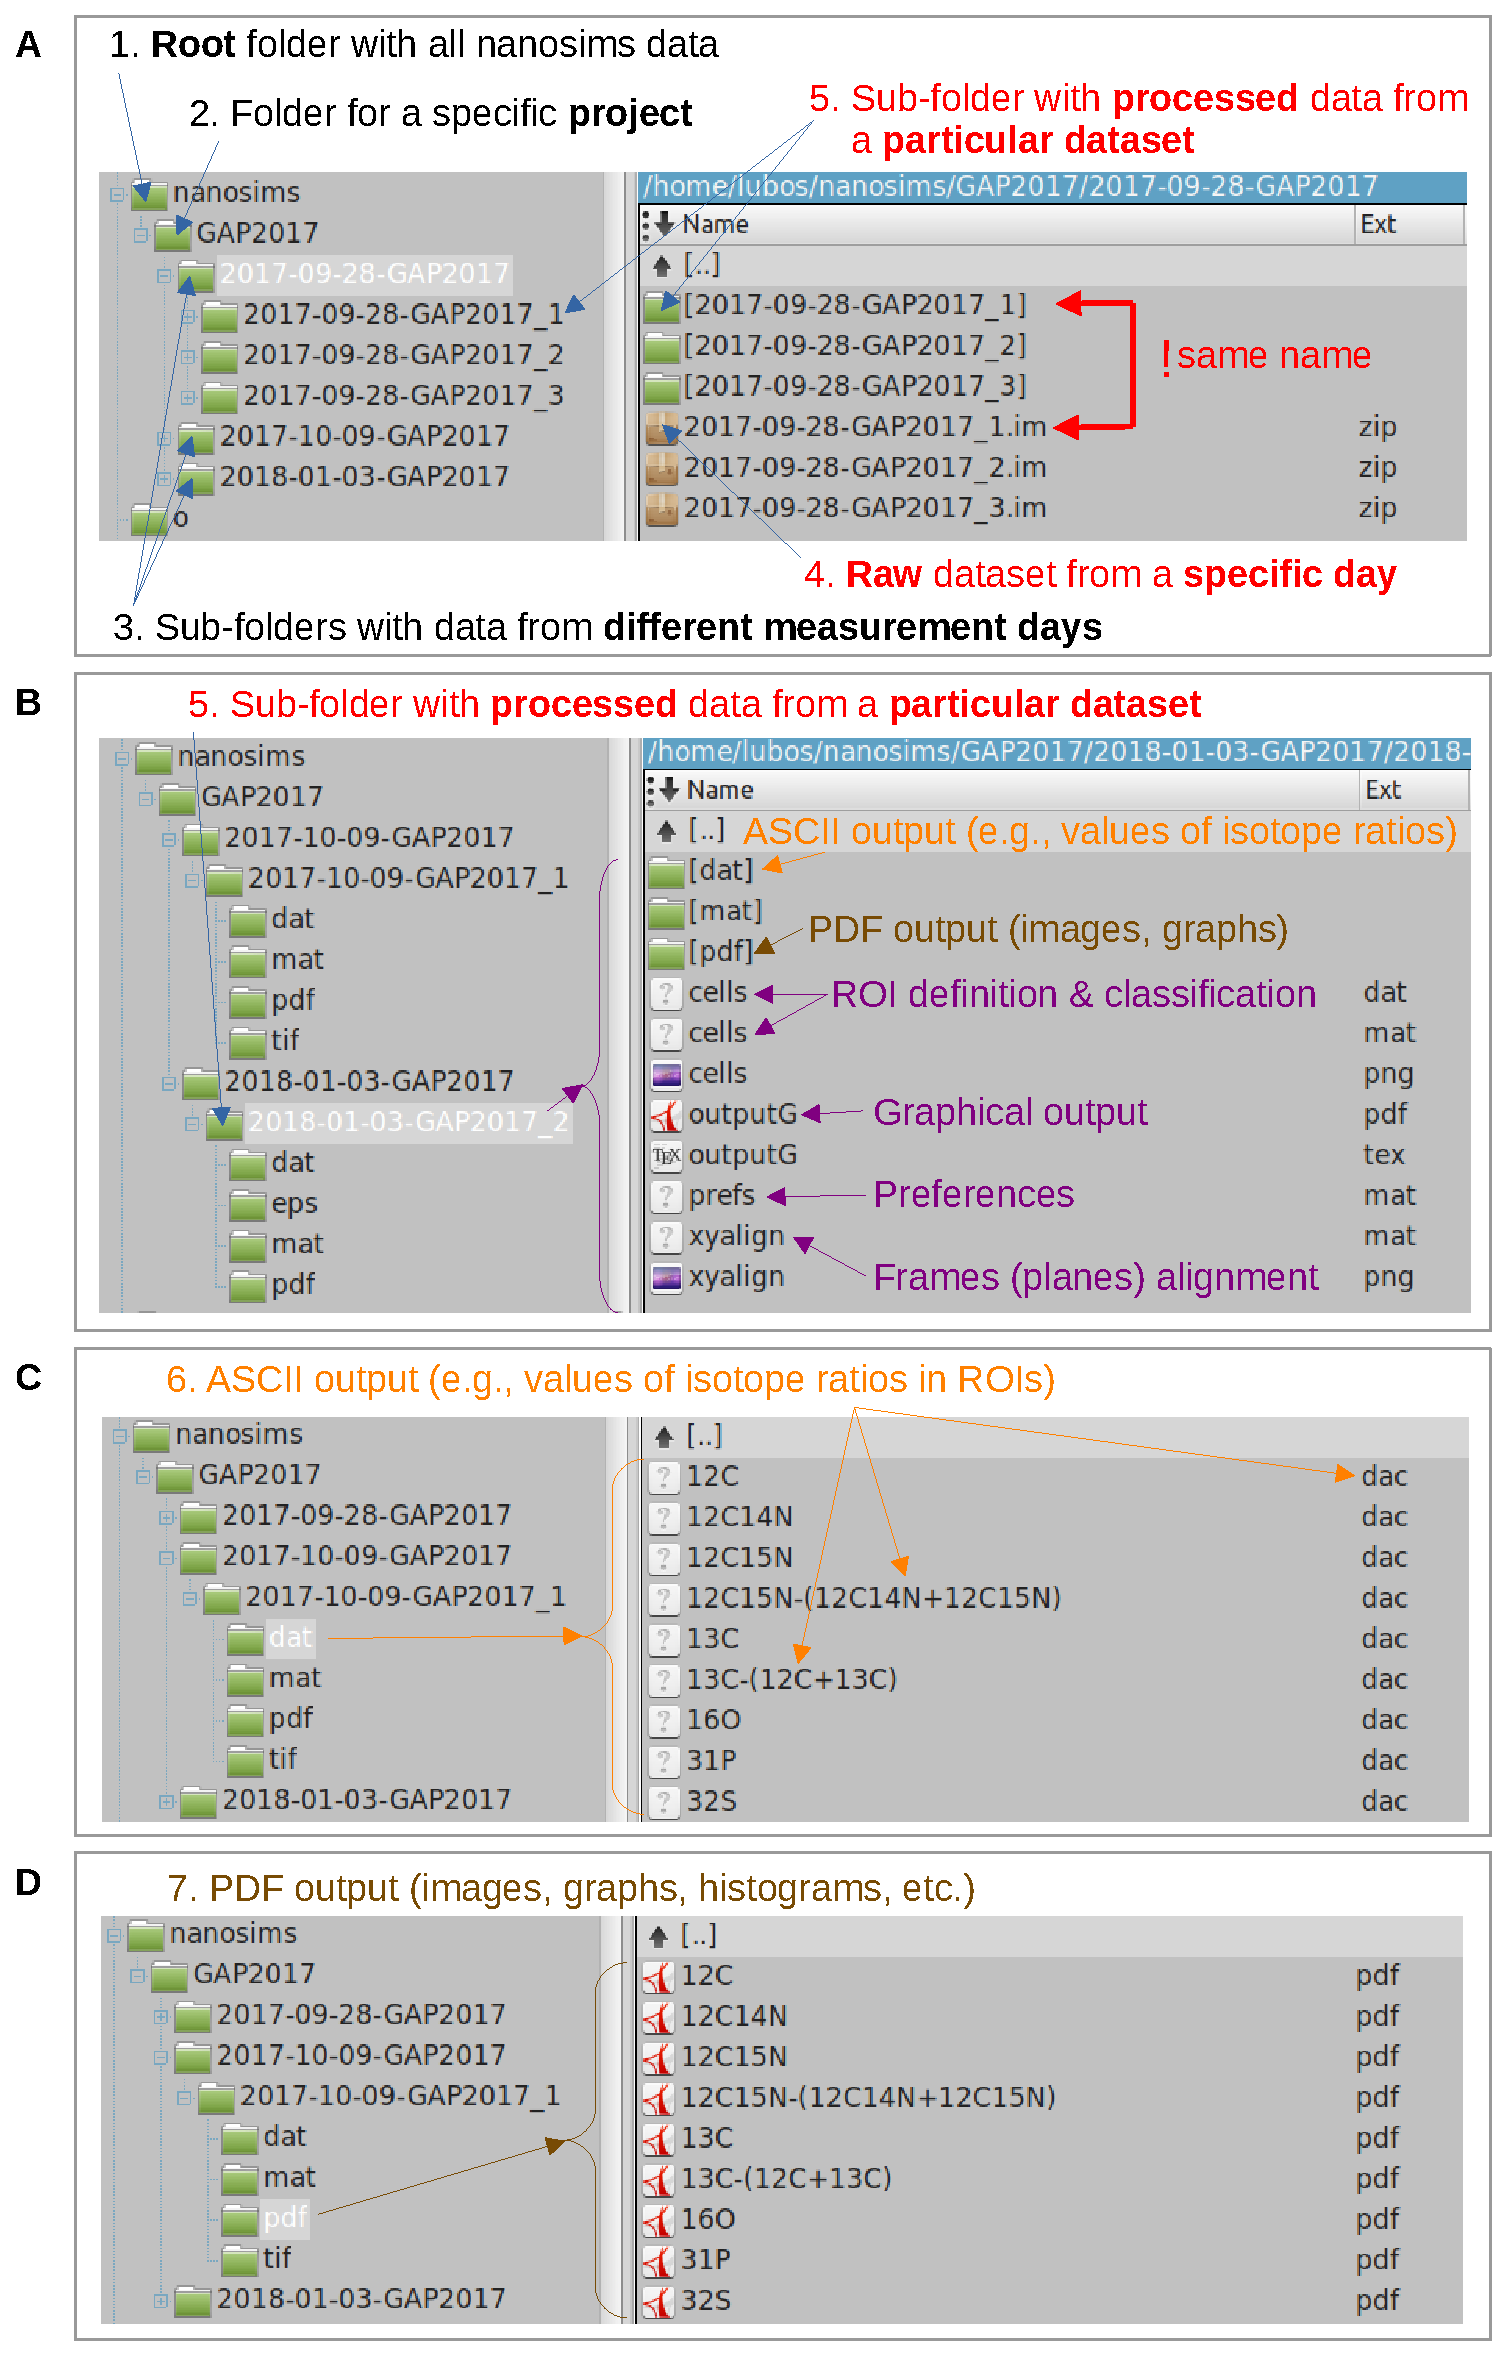
\includegraphics[height=0.97\textheight]{figs2/folders_organization}
%\caption[]{(see next page)}
%\end{figure}
%\begin{figure} [t!]
%    \captionsetup{labelformat=adja-page}
%    \ContinuedFloat
%    \caption[Figure]{%
%    Example of a hierarchical organization of the raw and processed nanoSIMS data implemented in Look@NanoSIMS. %
%    \textbf{(A)} The root folder (\ttt{nanosims}) contains a~project-specific sub-folder (\ttt{GAP2017}), which contains sub-folders with data measured on different days (e.g., \ttt{2017-09-28-GAP2017}, \ttt{2017-10-09-GAP2017}). %
%    The `day folder' contains \emph{multiple raw datasets} measured on that particular day (\ttt{im} or \ttt{im.zip} files). %
%    When a particular raw dataset is processed and analyzed, the data is stored in a `dataset folder' with the \emph{same name} as the dataset (see red `!'). %
%    \textbf{(B)} The `dataset folder' contains files defining the processing steps, including alignment information (\ttt{xyalign}), definition and classification of regions of interest (\ttt{cells.mat} and \ttt{cells.dat}, respectively), preferences (\ttt{prefs.mat}), and a comprehensive summary of results exported in a PDF file (\ttt{OutputG.pdf}). %
%    The `dataset folder' also contains sub-folders with ASCII (\ttt{dat}), PDF (\ttt{pdf}) and Matlab (\ttt{mat}) output. %
%    \textbf{(C)} The \ttt{dat} folder contains the ROI-specific ion counts and ion count ratios (\ttt{dac} files). %
%    \textbf{(D)} The \ttt{pdf} folder contains the exported images, graphs, histograms, etc. }
%    \label{fig2:data_organization}
%\end{figure}

\clearpage

\section{A typical data processing session with Look@NanoSIMS}

This section provides a \emph{quick summary} of steps taken during a typical data processing session with Look@NanoSIMS. Refer to Sections~\ref{sec:level1} and \ref{sec:level2} for more details, depending on the level of analysis. Throughout this document, we will use colored text when refering to a specific \lans{menu item or action button}, \lanscb{checkbox} or \lanstf{text field} in the program's GUI.


\subsection{Analysis of a single dataset --- starting from ``scratch''}
\label{sec:analysis_from_scratch}

The following steps will bring you from a raw dataset to basic output such as images or ROI-specific values of ion counts and ion count ratios. More details are provided in Section~\ref{sec:level1}.

\begin{enumerate}

\item Select \lans{Input} $\ra$ \lans{dead-time and QSA correction settings} to enable dead-time and QSA (quasi-simultaneous arrival) corrections.

\item Select \lans{Input} $\ra$ \lans{Load RAW dataset} to load raw data from disk. The raw data is stored in an \ttt{im.zip} or \ttt{im} file depending on whether it has been compressed or not.

\item Select \lans{Input} $\ra$ \lans{Autoscale plane images} to automatically set the scale for all masses. 

\item Select \lans{Input} $\ra$ \lans{Display plane images for all masses} to view the raw data as images, one plane at a time, displayed with a scale specified in the previous step. 

\item Define \lanstf{base mass for alignment} and then select \lans{Input} $\ra$ \lans{Display alignment mass} to check the data plane by plane, \lanscb{deselect planes} with artifacts or corrupt data, and \lans{define a region} for performing a drift-correction. 

\item Select \lans{Input} $\ra$ \lans{Accumulate plane images} to accumulate drift-corrected ion counts over selected planes.  

\item Select \lans{Input} $\ra$ \lans{Autoscale accumulated images} and then \lans{Input} $\ra$ \lans{Display accumulated images for all masses} to display the accumulated ion count images for all masses and export them in a PNG file.

\item Define \lanstf{expressions} for ion count ratios and the corresponding \lanstf{scales}. 

\item If you want to quantify ion counts and ion count ratios in regions of interest (ROIs), select \lans{ROIs} $\ra$ \lans{INTERACTIVE ROIs definition tool} to define the ROIs and store them on disk. Additionally, you can clasify the ROIs via \lans{ROIs} $\ra$ \lans{Classify} $\ra$ \lans{manually} or \lans{automatically}.

\item Select \lans{Output} $\ra$ \lans{Display masses} or \lans{Output} $\ra$ \lans{Display ratios} to perform various types of data analysis and visualization, including:

\begin{itemize}
\item display \lanscb{images}, \lanscb{depth profiles in ROIs}, \lanscb{lateral profiles}, or \lanscb{histograms},
\item \lanscb{combine images as RGB} overlays,
\item \lanscb{plot x-y-z graphs} (scatter plots) of ROI-specific ion counts or ratios,  
\item \lanscb{compare ROIs} with respect to ion counts or ratios using simple statistical methods.
\end{itemize}
%
Note that the appearance of the output can be tweaked via \lans{Preferences} $\ra$ \lans{Additional output options}.

\item Select \lans{Output} $\ra$ \lans{Generate LaTeX + PDF output} to export results of your analysis in a~comprehensive PDF file. 

\item Select \lans{Preferences} $\ra$ \lans{Store preferences} to save the settings of the current data processing session in a file (we recommend to use the file name \ttt{prefs.mat}). This is useful when you want to return to the analysis of the same file in the future, but also if you want to later combine results of your analyses of multiple datasets (``metafile processing''), as explained below. Therefore, it is highly recommended that you do this.

\item Optionally, select \lans{Preferences} $\ra$ \lans{Create full backup of processed data} to back up the processed data in a compressed (\ttt{zip}) file. This is useful for sharing the results of your data processing and analysis with collaborators.

\end{enumerate}

%%

\subsection{Continuation of a previously stored single-dataset analysis}

If you want to continue with the analysis of a dataset that you have analysed previously, you can save some time by following these steps:

\begin{enumerate}

\item Select \lans{Input} $\ra$ \lans{dead-time and QSA correction settings} to enable dead-time and QSA (quasi-simultaneous arrival) corrections.

\item Select \lans{Input} $\ra$ \lans{Load+accumulate+display RAW or PROCESSED dataset}. After you select the raw data and preferences files (\ttt{im.zip} or \ttt{im} file and \ttt{prefs.mat}, respectively), the data will be loaded, drift-corrected, accumulated and displayed automatically.

%\addon{You will be prompted to select the raw data (\ttt{im.zip} or \ttt{im} file) as well as the preferences file (e.g., \ttt{prefs.mat}). }

%\addon{After you do that, steps 2 (loading), 6 (drift-correction and accumulation) and 7 (display) described in Section \ref{sec:analysis_from_scratch} will be performed automatically.}
 
\item Select \lans{ROIs} $\ra$ \lans{Load ROIs from disk} to load the previously defined ROIs from disk.

%\addon{Choose the previously selected ROIs file, e.g., \ttt{cells.mat}. Modify ROIs definition or classification, if required.}

%\item Continue with steps 13--15 described in Section~\ref{sec:analysis_from_scratch}.

\end{enumerate}
%
After completing these steps, you can continue with further processing and analysis as described in the previous section (steps 8--13).

%%

\subsection{Analysis of multiple datasets --- ``metafile processing''}

After the analysis of several single datasets, you are left with isotope ratio values and images scattered across \emph{multiple} files and folders. You can quickly merge these multiple files into \emph{one} output file using the following steps. More details are provided in Section~\ref{sec:level2}.

\begin{enumerate}

\item Ensure that the raw and processed data are organized as described in Section~\ref{sec:data_organization} (see also Figures~\ref{fig2:data_organizationAB} and~\ref{fig2:data_organizationCD}).

\item Select \lans{Process multiple} $\ra$ \lans{Generate metafile} to define a list of datasets that will be analyzed together.

%\addon{Typically, the datasets selected in the list are part of a~project or correspond to a~particular set of treatments within a~project.}

\item Select \lans{Process multiple} $\ra$ \lans{Process metafile} to perform the analysis of multiple datasets.

\end{enumerate}
%
The output generated by metafile processing can be used for visualization and further analysis (e.g., statistical analysis) by LANS or other, third-party software.

%%

\section{A less common data processing in Look@NanoSIMS}

Over the years, different ways of analysis and visualization of nanoSIMS data have been added to Look@NanoSIMS. Although they may be useful only under special circumstances, it is good to know about them, just in case. They include:

\begin{enumerate}

\item \lanscb{Hue modulation} of ratio images based on a combination of mass images.

\item Integrating an \lans{external image} into the nanoSIMS dataset. This includes \lans{alignment} and \lans{overlays} of external and nanoSIMS images, definition of \lanstf{ROIs based on the external image}, and \lans{resampling} of nanoSIMS data to match the resolution of the external image.

\item Loading datasets in \lans{blocks}, including the possibility to load and combine \emph{multiple} raw datasets (measured in sequence) and analyze them as one dataset.

\item Visualization of \lanscb{lateral profiles across depth}.

\item Loading datasets with more than 8 masses. Such datasets can be acquired using the peak-switching mode, and they can contain up to 16 masses.

\item Automatic ROI classification.

\item Simple statistical analysis of ROI-specific ratios, including correlation, ANOVA, Kruskal-Wallis test.

\end{enumerate}
%
More details about these analyses are provided in Section~\ref{sec:level3}.

%%%%

\section{Analysis of a single dataset --- starting from ``scratch''}
\label{sec:level1}

This section describes in greater detail how to get from a raw dataset to basic output such as images or ROI-specific values of ion counts and ion count ratios. As an example, we will use the dataset \ttt{2017-09-28-GAP2017\_1.im.zip}.

\bb{Note:} When using Look@NanoSIMS, you will likely create many graphs and images, which may clutter your screen. Select \lans{Output} $\ra$ \lans{Close all figures} in the main GUI, or press~\ttt{Ctrl+g}, any time during the processing session to quickly close all figures at once.

\addtolength{\parskip}{2mm}

\subsection{Load nanoSIMS dataset from disk}

\s Select \lans{Input} $\ra$ \lans{Dead-time and QSA correction settings} to enable dead-time and quasi-simul\-ta\-neous arrival (QSA) corrections. Define the relevant parameters in the window that pops up (\figref). The corrections will be \bb{applied} based on these parameters \bb{during loading} of the raw data. Note that you can specify the parameters for up to 16 masses. This can be relevant if the dataset was acquired using a peak-switching mode.

\s Select \lans{Input} $\ra$ \lans{Ask for range of planes and masses before loading} if you want to interactively define \bb{a range of} planes and masses that should be extracted during loading of the raw dataset. This is unnecessary in most cases, but it may be useful if your dataset is huge (e.g., more than 1~GB of data) and the memory (RAM) on your computer is insufficient.

\s Select \lans{Input} $\ra$ \lans{Shift columns or rows when loading raw data}. This data correction is relevant for data acquired by the NanoSIMS 50L instrument at Utrecht University and probably very few others around the world. It concerns a glitch in the acquisition software, which causes the data in pixels from the first column (or row) to appear in the last column (or row), or vice versa. This option allows you to \bb{shift} the pixels to the \bb{correct} position during loading of the raw dataset. You can skip this step if this is not an issue in your dataset.

\s Select \lans{Input} $\ra$ \lans{Load RAW dataset} to load the raw dataset from disk in a standard way (i.e., plane by plane). When searching for the dataset, choose the file type: \ttt{im.zip} or \ttt{im}, depending on whether the raw data has been compressed or not. After selecting the raw data file, observe the progress of loading in the Matlab console. When the loading is finished, names of the masses will automatically be filled in the corresponding \lanstf{mass} text fields. Additionally, \ttt{[]} will be added in the \lanstf{planes} text field, which stands for ``all planes''.

\addon{Sometimes, the mass name entry in the binary \ttt{im} file is incorrectly saved. If this happens, a~``strange-looking'' name such as \ttt{au197} will be filled as the corresponding \lanstf{mass}, referring to the actual mass detected (in atomic units). If you know that the detected isotope was (in this example) ${}^{197}$Au, you can rewrite the string from \ttt{au197} to \ttt{197Au} and use it as the name of the mass in further analysis.}

%%

\subsection{Display of mass images plane-by-plane}

\setcounter{step}{0}

\s Select \lans{Input} $\ra$ \lans{Autoscale plane images} to automatically fill in the \lanstf{scale} for each detected mass. The scale, in the form of \ttt{[min max]}, is calculated as the 0.001 and 0.999 quantile of the ion counts across all pixels and planes. The quantiles can be adjusted using \lans{Preferences} $\ra$ \lans{Additional output options} (see Section~\ref{sec:AOO}). 

\s In the \ttt{Detected masses} box, check the \lanscb{checkboxes}  to the left from the \lanstf{masses} to select which masses will be displayed in the following step. By default, all masses are selected, but you may want to change it.

\s Select \lans{Input} $\ra$ \lans{Display plane images for all masses} to view secondary ion counts detected in individual planes for all masses (\figref). This is the actual data in its \emph{rawest} form, i.e., ion counts per pixel per plane.

\bul Use arrows to browse through the planes forward and backward.

\bul Click on \lans{Export as PNG} to export all masses in a particular plane as a PNG file. If you additionally check \lanscb{Export all}, you can export all planes, each into a separate PNG file.


When exploring the ion count images, you can often notice a small \bb{drift} when going from one plane to the next. This drift is caused by temperature instabilities during the measurements (a~bigger jump can also be caused by an~earthquake!). You will be able to correct for this drift in the next step. At this point, you should decide on the mass that will be used to calculate the drift correction (called \lanstf{Base mass for alignment}). As a~rule of thumb, it should be one with a relatively \bb{high ion counts} and \bb{clear contrast} across the image. In this example, it will be \ttt{12C14N}.

%%

\subsection{Drift-correction and accumulation of planes}
\setcounter{step}{0}

The drift-corrected accumulation of planes is controlled by settings specified in the \ttt{Accumulation options} box and by the numbers in the \lanstf{planes} list (Figure). 

\s Specify the \lanstf{Base mass for alignment}. This is done based on your choice made in the previous step (in this example: \ttt{12C14N}). 

\s Select \lans{Input} $\ra$ \lans{Display alignment mass}. 

\bul In the window that pops up (Figure), click on \lans{arrows} to browse through the individual planes. 

\bul Check \lanscb{Deselect} to mark the plane that should be excluded from accumulation (e.g., if the data in that plane is corrupt).

\bul After you have completed the plane selection or deselection, click on the \lans{Define alignment region} button to define an area in the image based on which the drift correction will be calculated in the next step. It is recommended to define this area as a~minimum rectangular region in the image that contains pronounced spatial heterogeneities (such as a cell or a group of cells). Close the window when you have defined the area.

\bul After you close the window, the x and y ranges of the alignment region will be written in the respective fields of \lanstf{Special region for alignment}. Also, the range of selected planes will be written in the \lanstf{planes} list. You can edit these fields if you know the correct values, but be careful not to make any syntax errors. 

\s Check \lanscb{Align images when accumulating} if you want to apply automated drift correction during the accumulation of planes. If not, which is rarely the case, leave this checkbox unchecked.

\s Select \lans{Input} $\ra$ \lans{Accumulate plane images} to start the accumulation of drift-corrected images. 

\bul You will be asked whether to employ a \lans{New} or \lans{Old} algorithm. In most cases, you will choose the new one. However, the old one is preferred if the drift-correction is based on images with very low ion counts (i.e., very pixelated images).

\bul Observe the drift-correction progress in the Matlab console. 

\bul When the drift-correction information is calculated for all selected planes, you will be prompted to accept or reject it. 

\bul If you \lans{accept} it, the information will be stored in the file \ttt{xyalign.mat} and all planes for all masses will be accumulated based on this information. Also, this information will automatically be used in the future if you load the raw dataset using \lans{Input} $\ra$ \lans{Load+accumulate+display RAW or PROCESSED dataset}.

\bul If you \lans{reject} it, you can reiterate the previous steps (1--4) until you arrive at a dataset with drift-corrected and accumulated planes.

\bul Note that you do need to accumulate the planes, because most of the subsequent data processing steps only work for the ion counts accumulated over all (selected) planes.

If you realize, anytime at a later point during your data processing, that you are not satisfied with the drift-correction, you need to first delete the \ttt{xyalign.mat} file (via \lans{Preferences} $\ra$ \lans{Remove xyalign.mat from disk}), then \lans{Load RAW dataset}, and then repeat the previous steps (1--4) to drift-correct and accumulate the planes again.

%%

\subsection{Display accumulated mass images}
\setcounter{step}{0}

\s Select \lans{Input} $\ra$ \lans{Autoscale accumulated images} to update the \lanstf{scale} fields with a range optimized for displaying accumulated mass images. 

\bul The optimum scale is calculated as the 0.001 and 0.999 quantiles of the accumulated ion counts across the image pixels. These quantiles can be adjusted via \lans{Preferences} $\ra$ \lans{Additional output options}.

\s Alternatively, define the \lanstf{scale} \bb{manually} by typing in the \ttt{[min max]} (minumum and maximum) values by yourself. If you then press \ttt{Enter}, the corresponding mass will be displayed in a new window using the color scale defined by the specified range. You can repeat this many times to \bb{quickly adjust} the color scale for optimal display.

\bul Note that you can display the images in multiple colormaps. These can be adjusted via \lans{Preferences} $\ra$ \lans{Additional output options} (see Section~\ref{sec:AOO}). Explore them to find the best you like. If you want to display the images in grayscale, click on the corresponding \lanscb{B\&W} checkbox next to the scale.

\bul If there is a large contrast in ion counts across the image, it is often useful to display the log-transformed image. To do this, check \lanscb{Log10-transform} in the \ttt{Output options} box before you press \ttt{Enter} to display the image. When displaying log-transformed images, make sure that the minimum value of the \lanstf{scale} is greater than 0. If it is 0 and you press \ttt{Enter}, the image will be displayed in a~scale where $\ttt{min} = 0.001\times\ttt{max}$, which may not be optimal.

\s Select \lans{Input} $\ra$ \lans{Display accumulated images for all masses} to display the images, lumped together for all masses, and
export them in a PNG file.

\s Check \lanscb{Display images} in the \ttt{Output options} box and then select \lans{Output} $\ra$ \lans{Display masses} to display the images in a nicer way and separately for each mass. 

\bul In this step, the image appearance, including the location of the colorbar, size and location of the scale bar, etc., can be tweaked via \lans{Preferences} $\ra$ \lans{Additional output options} (see Section~\ref{sec:AOO}). 

\bul Ensure that \lanscb{Export PDF graphics} in the \ttt{Output options} box is checked to export the images as PDF (in the \ttt{pdf} sub-folder of the current data folder).

%%

\subsection{Display ratio images}
\setcounter{step}{0}

\s Type \bb{formulas} for calculating ratio images in the  \lanstf{expression} fields. In principle, the formula can be any valid arithmetic expression containing any of the detected masses. However, it is recommended not to make the formulas too complicated. Typical examples include:

\begin{itemize}
\item \ttt{13C/12C} to calculate the $^{13}C/^{12}C$ isotope ratio,
\item \ttt{13C/(12C+13C)} to calculate the $^{13}C$ atom fraction,
\item \ttt{32S/12C} to calculate the $^{32}S/^{12}C$ ion count ratio (a proxy for the S/C elemental ratio), 
\item \ttt{19F/plane} to calculate the average $^{19}F$ ion counts per detected plane, 
\item \ttt{19F/plane/pixel} to calculate the average $^{19}F$ ion counts per plane per pixel (only applicable if ROIs are defined; see below).
\end{itemize}

\s For each expression, type in the \lanstf{scale} to the correspoding field. Similar to masses, the scale should be in the form \ttt{[min max]} (minumum and maximum). 

\bul If you then press \ttt{Enter}, the corresponding ratio image will be displayed in a~new window using the color scale defined by the specified range. You can repeat this many times to \bb{quickly adjust} the color scale for optimal display.

\s Check \lanscb{Display images} in the \ttt{Output options} box and then select \lans{Output} $\ra$ \lans{Display ratios} to display the ratio images.

\bul In this step, the image appearance can be tweaked via \lans{Preferences} $\ra$ \lans{Additional output options}.

\bul Ensure that \lanscb{Export PDF graphics} in the \ttt{Output options} box is checked to export the images as PDF.

%%

\subsection{Display RGB overlays}
\setcounter{step}{0}

To increase the information value of the mass and ratio images, they can be combined and displayed as RGB overlays.

\s To specify which image will be filled in the red, green and blue channel of the RGB overlay, enter identification numbers (1--8, found to the left of the mass names or ratio expressions) in the corresponding \lanstf{R/x}, \lanstf{G/y} and \lanstf{B/z} fields (found under \ttt{Plot-x-y-z graph} in the \ttt{Output options} box).

\bul At most one number per R, G and B field is allowed. If one or more of the fields is left empty, the corresponding channel(s) will be set to zero and thus appear black in the RGB overlay.

\s In the \ttt{Output options} box, check \lanscb{Combine images as RGB}. Then, check \lanscb{Pixel by pixel} to combine the images without modification and/or \lanscb{ROI-averaged} to use ROI-averaged values when creating the overlays (the latter is only possible if ROIs have been defined).

\s Select \lans{Output} $\ra$ \lans{Display masses} or \lans{Display ratios} to display the RGB overlay derived from mass or ratio images, respectively.

\bul If you want to overlay a~mass image with a~ratio image, enter
the corresponding name of the mass into one of the \lanstf{expression} fields, specify the scale, enter the corresponding identification number in one of the \lanstf{color} fields (R, G or B), and then select \lans{Output} $\ra$ \lans{Display ratios}. 

\bul You can combine multiple masses with multiple ratios by entering the corresponding identification numbers in the R, G and B fields.

\bul In addition to PDF, RGB overlay images are also exported as TIF files (in the \ttt{tif} sub-folder of the dataset folder).

%%

\subsection{Define ROIs}
\setcounter{step}{0}

Typically, much of nanoSIMS data analysis revolves around regions of interest (ROIs). There are many options for defining ROIs in Look@NanoSIMS, as described below. Once you get used to it and learn the ``tricks'', ROI definition can be very efficient. 

We re-emphasize the importance of looking at the comments written in the Matlab console while defining ROIs. They provide more details about what to do while performing specific steps. The key constraint is: if you start an action, you \emph{must} finish it. If you don't, the program will likely get ``stuck'' and you may need to terminate it. We won't go into details here, but briefly, this peculiarity is related to the way Matlab handles user's input in a drawing mode. Thus, beware and keep an eye on the messages in the console. You can also learn more about this topic via \lans{Help} provided in the ROI definition tool window.

\s In the main Look@NanoSIMS GUI, specify the \lanstf{ROI definition template}. 

\bul This can be an individual mass, ratio, an RGB overlay of masses or ratios, or an external image.

\bul In this example, we will use an RGB overlay of \ttt{12C15N/12C14N}, \ttt{12C14N} and \ttt{31P}. Since we want to combine ratios and masses, we enter \ttt{12C14N} as expression \#3, \ttt{31P} as expression \#4, and copy the scale for both in the corresponding \lanstf{scale} field. Then, we enter \ttt{2}, \ttt{3} and \ttt{4} to the fields for \lanstf{R}, \lanstf{G} and \lanstf{B}, respectively. Finally, we enter \ttt{rgb2} as the \lanstf{ROI definition template} (entering \ttt{rgb} means that we use an RGB overlay, \ttt{2} means that we use an overlay of ratios rather than masses).

\bul The ROI template can optionally be \bb{smoothed} before it is used for ROI definition. Smoothing is done using a median filter with a~two-dimensional kernel size (in pixels) specified in the \lanstf{Smoothing kernel} field. If applied, ROI outlines will generally be smoother if defined using the \lans{interactive thresholding} approach (see below). In this example, we will not do any smoothing and just use \ttt{[1 1]} as the smoothing kernel.

\s Select \lans{ROIs} $\ra$ \lans{Display template for ROI definition} to verify that the template looks as intended. 

\s Select \lans{ROIs} $\ra$ \lans{INTERACTIVE ROIs definition tool} to open a~window dedicated to ROI definition (Figure). 

\bul During this process, you will be prompted to select the \ttt{ROI file} (e.g., \ttt{cells.mat}) and \ttt{ROI classification file} (e.g., \ttt{cells.dat}). Select them if the files have been previously created and you want to reuse them, or press \lans{Cancel} if they do not exist (yet).

\bul If they exist and you do select them both, they will be \bb{linked}. This means that when you add or remove a~ROI from the image file, the corresponding ROI will also be added or removed from the classification file.

After these steps, a new window (\ttt{ROIs definition tool}, Figure) will open, allowing you to define, display and save ROIs using the various menu items.

\setcounter{step}{0}

\s Select \lans{Action} $\ra$ \lans{Draw ROIs freehand} (\ttt{Ctrl+D}) to draw a ROI using a mouse.

\bul Click the left mouse button, hold it, and draw a region of interest. 

\bul After releasing the mouse button, you can move the ROI around using a mouse. 

\bul Double-click on the ROI to confirm its final position.

\bul When prompted, specify whether the ROI outline should be defined as the \lans{coarse polygon} you have just drawn or as an \lans{ellipse that circumscribes} this polygon. Typically, you will choose the first option: coarse polygon.

\s Experiment with different ways of defining ROIs, including drawing them as \lans{ellipses} (\ttt{Ctrl+E}) or \lans{rectangles} (\ttt{Ctrl+t}).

\bul You always need to double-click on the ROI to confirm its size and location.

\bul Note that if you draw a ROI over another, previously defined ROI, the last one will take the priority. In this way, you can draw ROIs inside ROIs.

\s Select \lans{Action} $\ra$ \lans{Interactive thresholding} (\ttt{Ctrl+A}) to define a ROI more efficiently. 

\bul This approach is only applicable if the signal used for recognizing the ROI stands out relative to the surrounding background.

\bul After invoking \lans{Interactive thresholding}, click with a~left-mouse button on the image in a~pixel with a~high signal. You will notice that a~ROI outline is automatically drawn. The outline corresponds to a~contour where the signal values do not fall below the value in the selected (clicked) pixel multiplied by a~threshold value.

\bul This threshold value is 0.5 by default, but it can be changed interactively by pressing the \lans{up} or \lans{down} arrow key, respectively. When doing so, the ROI outline will cover a~larger or smaller area. If a~different pixel is selected (clicked), the ROI outline is automatically redrawn according to the current threshold. By combining left mouse clicks with the \lans{up} and \lans{down} arrows, you can rapidly optimize the ROI definition.

\bul When you are satisfied with the defined ROI, press \ttt{Enter} to confirm it. Press \ttt{Esc} if you want to cancel the current interactive ROI definition.

\bul \bb{Note 1:} This is one of the moments when you can get stuck, and become unnecessarily frustrated, if you do not correctly follow the sequence of steps described above. Specifically, if you start the \lans{Interactive ROI definition} sequence of actions, you \emph{must} terminate it properly by pressing either \ttt{Enter} (confirm the ROI) or \ttt{Esc} (cancel the interactive ROI definition). 

\bul \bb{Note 2:} It is recommended that you spend some time practicing the above Interactive thresholding sequence. Once you get used to it, it can fairly substantially speed up your ROI definition.

\bul When an RGB overlay is used as a template for ROI definition, as in this example, the color channel used for automatic ROI drawing can be changed via \lans{Select interactive channel} $\ra$ \lans{red}, \lans{green} or \lans{blue}. Also, any of the RGB channels can be shown or hidden via \lans{Select interactive channel} $\ra$ \lans{red  shown}, \lans{green shown} or \lans{blue shown}. Use the hotkeys \ttt{Ctrl+1}--\ttt{Ctrl+6} to access these options quickly.

\s Select \lans{Display ROIs} $\ra$ \lans{Display ROIs with ROI ID's} (\ttt{Ctrl+w}) to display the currently defined ROIs.

\bul The newly opened window will be placed just to the right from the window of the ROIs definition tool. Thus, it is recommended that you keep the latter window somewhere on the left side of your screen. If you had placed that window near the right edge of your screen, it may happen that the window with the ROIs will be invisible (because it will be placed to the right of the tool window, i.e., outside of your screen).

\bul Notice that ROI identification numbers (ID's) are generated automatically and increase from left to right when sorting the ROIs based on their central point.

\bul If you want to display ROIs with specific ID's, you can do so by typing the ID's in the dialog that opens after you choose to display the ROIs.

\bul If the ROIs have been classified, you can display only ROIs of a~specific class by typing the corresponding class identification letter, rather than the ROI identification number, in the same dialog.

\s Explore the \lans{Action} menu to test various ways to \lans{define}, \lans{split}, \lans{merge}, or \lans{remove} ROIs (Figure).

\s Use the \lans{Zoom} menu to zoom in the ROI definition image or zoom out.

\bul Note another Matlab-related peculiarity: Once you select \lans{Zoom} $\ra$ \lans{Zoom ENABLE} (\ttt{Ctrl+z}), you enter a~`zoom' mode. In this mode, you can use the mouse to specify the zoomed-in area. Subsequently, you must quit the `zoom' mode by selecting \lans{Zoom} $\ra$ \lans{Zoom DISABLE} (or pressing \ttt{Ctrl+z} again). Only then can you proceed with other actions.

\s Select \lans{Save ROIs} from the menu, or press \ttt{Ctrl+s}, to save the currently defined ROIs. 

\bul You can choose the default name (e.g., \ttt{cells.mat}) or a different name.

\bul Note that there is no \ttt{undo} function implemented in Look@NanoSIMS (yet). Thus, it is recommended that you save the ROIs frequently, or at least after you have made an effort to define a~few complicated ROIs that you do not want to loose.

\s When you are satisfied with the defined ROIs, display them all again by selecting \lans{Display ROIs} $\ra$ \lans{Display ROIs with ROI ID's} (\ttt{Ctrl+w}). This will set the floor for the next step, the ROI classification.

%%

\subsection{Classify ROIs}

It is often useful to classify the defined ROIs. It is recommended to classify the ROIs \bb{after} the ROI definition has been fully completed and quality checked. This is because ROI definition, when performed with a~linked ROI classification file, is still not completely bug-free and may lead to a~mismatch between defined and classified ROIs after splitting a~ROI to multiple ROIs.

ROIs can be classified manually or automatically. Here, we focus on manual ROI classification, which is done in most cases. Automatic ROI definition will be explained in Section~\ref{sec:manual_ROI_classification}.

\bb{Note:} ROI classes in Look@NanoSIMS are identified by \bb{single} letters (e.g., \ttt{a}, \ttt{b}, \ttt{A}, \ttt{B}). Upper-case and lower-case letters refer to \emph{different} classes. It is up to the user to keep track of the full class name (e.g., algal cell, bacterial cell, filter) and the corresponding class identifier (e.g., \ttt{a}, \ttt{b}, \ttt{x}). Also, it is not recommended to use a~class identifier \ttt{i}, since this letter is automatically assigned to ROIs inserted to a~previously defined and classified set of ROIs.

\setcounter{step}{0}

\s While having the ROIs displayed, select in the main Look@NanoSIMS window \lans{ROIs} $\ra$ \lans{Classify} $\ra$ \lans{Manually}.

\s In the new window that pops up, specify the \lanstf{number} identifying the ROI and the corresponding \lanstf{letter} identifying the class in the fields provided, then click \lans{Add/Replace} (or press \ttt{Ctrl+Enter}). 

\bul Notice that after you add the classified ROI, the ROI identifier number is automatically increased by one and the ROI class letter is highlighted. This allows you to simply type in another (or the same) letter and press \ttt{Ctrl+Enter} to classify the subsequent ROI. By repeating this, you can fairly quickly classify many ROIs.

\bul Ensure that you correctly add the \emph{last} ROI to the list of classified ROIs. It often happens that users forget this and end up with one less ROI classified than defined, which causes errors later on.

\s Click on \lans{Save ROIs as} to store the ROI classification information in a~file. It is important, but also logical, that the filename (not the extension, see next) will be the same as the name of the ROI definition file. For example: if ROIs are stored in \ttt{cells.mat} or \ttt{ROIs.mat}, the corresponding classes should be stored in \ttt{cells.dat} or \ttt{ROIs.dat}, respectively.

\s Revise the ROI classification. If you need to change a ROI's class, click on the ROI identifier number, change its class, and click on \lans{Add/Replace} (or press \ttt{Ctrl+Enter}) to update it.

\s Click on \lans{Save ROIs} to store the ROI classes in the same file as defined via \lans{Save ROIs as} (Step~3).

\s Close the ROI definition and ROI classification windows when finished with the definition and classification tasks.

%%

\subsection{Display and export ROI-specific data}
\setcounter{step}{0}

\s Ensure that ROIs have been defined and, if required, classified.

\bul If ROIs have been defined in an earlier Look@NanoSIMS session, you first need to load them via \lans{ROIs} $\ra$ \lans{Load ROIs from disk}.

\s Check \lanscb{Plot x-y-z graph} in the \ttt{Output options} box and type identifiers (1--8) of the masses or ratios that you want to include in a~scatter plot in the \lanstf{R/x}, \lanstf{G/y} and \lanstf{B/z} fields. 

\bul If all three fields are filled in, the ROI-specific values will be plotted in a~3D scatter plot (x--y--z). If only two of the three fields are filled in, a~2D scatter plot (x--y) will be created.

\bul In the \ttt{Ratios} or \ttt{Detected masses} box, ensure that the checkboxes corresponding to the identifiers filled in the \lanstf{R/x}, \lanstf{G/y} and \lanstf{B/z} fields are checked, too. 

\s Check \lanscb{ROI-averaged} or \lanscb{Pixel by pixel} (also in the \ttt{Output options} box) if you want to display a~scatter plot for ROI-specific or pixel-specific values, respectively.

\bul You can have both of them checked at the same time. 

\s Check \lanscb{Export ASCII data} and \lanscb{Export PDF graphics} to ensure that the data and graphs will be exported (in the \ttt{dat} and \ttt{pdf} sub-folders of the dataset folder, respectively).

\s When plotting scatter plots, it is typically not necessary anymore to display the corresponding images. If this is the case for you, uncheck the \lanscb{Display images} checkbox.

\s Select \lans{Output} $\ra$ \lans{Display masses} or \lans{Display ratios} to create scatter plots of the ROI-specific or pixel-specific values of the desired quantities and export the values and graphs. 

\bul In the process, you will be prompted to select a~ROI classification file. If the file exists (and it is up-to-date), select it. In this case, different colors will be used to mark ROI from different classes. 

\bul If the ROI classification file does not exist, click \ttt{Cancel} or press \ttt{Esc} when prompted for the file. In this case, all ROIs will be treated equally and displayed in one color.

\bul If you only want to display values for specific classes, you can enter the identifiers for those classes in the \lanstf{For classes} field (just below the R/x, G/y and B/z fields) first, then select \lans{Output} $\ra$ \lans{Display masses} or \lans{Display ratios}.

\bul If you choose to display ROI-specific values, it is possible to add a~ROI identifier and an~error-bar to each data point. This is achieved by selecting the corresponding options via \lans{Preferences} $\ra$ \lans{Additional output options}. The error-bar size will indicate the Poisson error, derived from the total ion counts per ROI.

\bul The output data and images will be stored in the \ttt{dat} and \ttt{pdf} sub-folders of the dataset folder, respectively. Formatting of the data output is explained in Section~\ref{sec:DataOutputFormat}.

\s Select \lans{Output} $\ra$ \lans{Check output consistency} to check that the exported ROI-specific data are consistent with the defined ROI  classes (only relevant if working with classified ROIs). 

\bul More specifically, the output is consistent if the number of defined ROIs, the number of classified ROIs, and the number of ROIs for which the ROI-specific data have been exported, is the \emph{same}.

\bul Output inconsistency can occur if, e.g., you redefine ROis but forget to reclassify them or reexport the ROI-specific data (or any combination of these three actions).

\bul When prompted, select the ROI classification file and observe the results of the consistency chek in the Matlab console. 

\bul If any of the output lines does not contain \ttt{OK}, you should revise your analysis by reclassifying the ROIs or reexporting the ROI-specific data for the affected variables.

%%

\subsection{Display depth profiles in ROIs}
\setcounter{step}{0}

NanoSIMS measurements are conducted by sputtering away the sample material in multiple scans over the same field of view while collecting the ion counts. The resulting image stack therefore reflects elemental and isotopic distribution of the sample along the vertical dimension. You can easily display and export this vertical (depth) variation in ROIs using the following steps.

\s Ensure that ROIs have been defined or loaded into the current Look@NanoSIMS session.

\s Check \lanscb{Display depth profiles in ROIs} in the \ttt{Output options} box.

\bul Typically, you will want to uncheck all other checkboxes in the \ttt{Output options} box to prevent cluttering of your screen with too many figures.

\s Check \lanscb{Detected masses} or \lanscb{Ratios} for which you want to have the depth profiles displayed.

\s Select \lans{Output} $\ra$ \lans{Display masses} or \lans{Display ratios}.

\bul Observe the output in the Matlab console, which informs you about significant trends with depth of the particular mass or ratio in ROIs.

\bul In the process, the depth profiles are exported in data files with an extension \ttt{dap} (located in the \ttt{dat} sub-folder of the dataset folder).

\s In the new window that pops up, select ROI identifiers for which you want to display the depth profiles. Then, select the mass or ratio in the list for which you want to display the depth profiles.

\s Select \lans{Export depth profile} to export the graph with depth profiles in the currently selected ROIs.

%%

\subsection{Finalize the processing of an individual dataset}
\setcounter{step}{0}

If you want to reprocess a~particular dataset in the future and start the processing from the same stage where you finished, you will need to have the data processing settings stored. If you want to share or communicate the results with collaborators, a~graphical output where all the images and graphs generated by Look@NanoSIMS are nicely assembled next to each other might be a~good idea. Finally, if you want to make a~backup of the processed data for yourself or for sharing with collaborators, having a~compressed version of the processed data folder would probably be the best approach. You can generate these types of output quickly and efficiently within Look@NanoSIMS using the following steps:

\s Select \lans{Output} $\ra$ \lans{Generate LaTeX + PDF output} to export results of your analysis in a~PDF document. 

\bul Before you do this, check boxes in the \ttt{Output options} box to specify which kind of results you want to have included in the graphical output, including  \lanscb{images}, \lanscb{scatter plots}, \lanscb{histograms}, or \lanscb{depth profiles}.

\bul If you check \lanscb{View PDF after export} (available via \lans{Preferences} $\ra$ \lans{Additional output options}) and correctly set the full path to a~PDF viewer in the \ttt{PDF\_VIEWER} variable (this variable is defined in the \ttt{lans\_paths.m} file), the PDF output will automatically be displayed after it has been generated. This can be convenient if you want to see the results quickly, without the need for browsing through the different folders on your computer.

\s Select \lans{Preferences} $\ra$ \lans{Store preferences} to save the settings of the current data processing session in a file (we recommend to use the file name \ttt{prefs.mat}). 

\bul This is useful when you want to return to the analysis of the same file in the future, but also if you want to later combine results of your analyses of multiple datasets (``metafile processing''), as explained below. Therefore, it is highly recommended that you do this for every processed dataset.

\bul More specifically, the preferences file will contain all information for the currently processed dataset that you see in the main window of Look@NanoSIMS, including the names of detected masses, planes selected for alignment, formulas for ion count ratios, scales for mass and ratio images, output options, etc.

\s Select \lans{Preferences} $\ra$ \lans{Backup (full) folder with processed data}.

\bul This will compress the \emph{entire} content of the processed data folder in a~\ttt{zip} file.

\bul Additionally, a~copy of the PDF output file will be created and renamed to match the name of the processed data.

\s Alternatively, select \lans{Preferences} $\ra$ \lans{Backup (minimal) folder with processed data}.

\bul This will only compress the \emph{minimal} information in the processed data folder, based on which the rest of the processed data can easily and reproducibly be generated by repeating the processing steps in Look@NanoSIMS. 

\bul This minimal information includes the preferences (e.g., \ttt{prefs.mat}), plane alignment information (\ttt{xyalign.mat}), ROI definition (e.g., \ttt{cells.mat}), and ROI classification (e.g., \ttt{cells.dat}).

%%

\section{Analysis of multiple datasets --- ``metafile processing''}
\label{sec:level2}

It is assumed that you have processed multiple NanoSIMS datasets using steps described in Section~\ref{sec:level1}, which left you with output such as isotope ratio values and images scatterred across multiple files and folders, organized as described in Section~\ref{sec:data_organization}. This section explains how to quickly merge these multiple files into \emph{one} output. If you are a~skilled data analyst, you can arguably do this more efficiently by creating scripts in a~programming language of your choice. This section describes how to do this in Look@NanoSIMS, if your coding abilities are more limited.

%%%%

\subsection{Generate metafile}
\setcounter{step}{0}

The first step involves the definition of a~list of datasets and variables that you want to merge and analyze together. In the context of Look@NanoSIMS, this list is stored in a~so-called metafile, which is a~simple text file containing the required information including the absolute path to the processed data structure, relative paths for the individual datasets, and variables of interest. This file can be generated in a~simple text editor, but it is better to start using a~dedicated tool in Look@NanoSIMS to avoid syntax errors.

\s From the menu in the main LANS window, select \lans{Process multiple} $\ra$ \lans{Generate metafile} to open a~new tool window dedicated to metafile definition (Figure). 

\s In this tool window, click on \lans{Select base folder} to select the absolute path to the processed datasets.

\bul It is assumed that the folders with the processed datasets are located in this path or in subfolders under it.

\s Click on \lans{Select dataset}, navigate to a~specific processed dataset, and select it.

\bul You need to select the raw data file (\ttt{im} or \ttt{im.zip} file), not the sub-folder containing the processed data. However, the corresponding sub-folder with the processed data must exist.

\bul You can select multiple datasets at once, using the \ttt{Ctrl} key. 

\s Enter a~\lanstf{treatment identifier} to the provided field.

\bul This must be an \emph{integer number}, e.g., $0$ for a~control treatment, $1$ for treatment~\#1, etc.

\s Enter \lanstf{ROI classes} you want to analyze via metafile processing in the provided field.

\bul Enter \ttt{*} if you want to analyze all ROI classes, unless you really only want to analyze ROIs from a~specific class. Note that you will be able to make this selection later on anyway, so it is best to simply enter \ttt{*}.

\s Click \lans{Add} to add the dataset to the list. 

\s Repeat steps 3--6 to select all datasets that should be part of the metafile processing.

\bul If you want to remove a dataset from the list, select it in the list and then click \lans{Remove}.

\s In the fields provided, enter \lanstf{variables} that you want to analyze via metafile processing. 

\bul Ensure that you type the strings \emph{exactly} in the same way as you did during the processing of individual datasets (e.g., \ttt{13C/12C}, \ttt{13C/(12C+13C)}, \ttt{12C15N/12C14N}, \ttt{31P/plane/pixel}, etc.). Best is to copy and paste the strings from the main LANS window to avoid typos.

\bul You can analyze up to six variable simultaneously. The idea behind this limit is that you can, later on, plot the variables against each other in up to three 2D-scatter plots or up to two 3D-scatter plots. Thus, it is good to think ahead and enter the variable in the order how you will want to plot them later on, e.g., \ttt{13C/12C} as variable~1 (later $x$), \ttt{12C15N/12C14N} as variable~2 (later $y$), etc.

\s Click \lans{Save metafile} and define the name and location for the metafile.

\bul Ideally, to keep everything well organized, the metafile should be located in the \lanstf{base folder} selected above. 

\bul For example, if you call the metafile \ttt{mf1.txt}, any output generated during processing of this metafile will be stored in a~sub-folder called \ttt{mf1}.

\s Optionally, explore the content of the metafile by opening it in a~simple text editor.

\bul This is recommended because, later on, you may find it easier to edit the content of this file (e.g., add or remove datasets, modify the variables) directly in the editor rather than through steps 2--8 described above.

%%

\subsection{Process metafile}
\setcounter{step}{0}

\s Ensure that the metafile is defined and the sub-folders and corresponding output files exist and are consistent for all datasets listed in the metafile.

\bul This should be the case if you conducted the data processing attentively and in accordance with instructions described in Section~\ref{sec:level1}. If there are inconsistencies, they will be reported later on in the console (see below).

\s In the main LANS window, select \lans{Process multiple} $\ra$ \lans{Process metafile} to open a~new tool window dedicated to metafile processing.

\s In this tool window, select the \lanstf{base folder}.

\bul Typically, this folder will be the same as specified during metafile definition. However, if you reorganized the data on your computer, or if you conduct the metafile processing on a~different computer, the data organization may be quite different. Thus, this feature makes the metafile processing more portable across different computers.

\s Select the \lanstf{metafile}.

\s Specify  the \lanstf{scale}, separately for each variable.

\bul If specified in the form of \ttt{[min max]}, corresponding to a~minimum and maximum value, the scale will be applied during the following analyses. For example, images for the corresponding variable will be reexported as PDF using this new scale, or scatter plots containing the variable will apply this new scale.

\bul However, since the optimal scale for the images or graphs may initially be unknown, it is a~good idea to start with an empty scale, indicated by \ttt{[]}. This will have no effect on the displayed graphs or images for the corresponding variable.

\s Check \lanscb{log} if you want the variable to be log-transformed before display, separately for each variable.

\s Specify the mapping between ROI classes and \lanstf{colors} and between treatments and \lanstf{symbols} in the respective fields. 

\bul This mapping will be applied when plotting scatter plots.

\s Save the metafile processing settings using \lans{Action} $\ra$ \lans{Save settings}.

\bul This is useful if you plan to return to the same metafile processing session in the future.

\bul Once save, the settings can be loaded using \lans{Action} $\ra$ \lans{Load settings}.

Subsequent metafile processing analyses depend on your preferences and include several possibilities, as described next. 

\subsubsection{Export images for selected variables}
\setcounter{step}{0}

\s Select \lans{Action} $\ra$ \lans{Export images separately for each variable}. 

\bul This action will combine images of the variables from multiple datasets and export them in a~PDF output, \bb{one file per variable}. This allows you to view all images from a~specific project in one place, which is useful for a~visual comparative analysis.

\bul The visual comparison can be made easier if all images are displayed in the same scale. This is achieved by setting the minimum and maximum values in the corresponding \lanstf{scale} field, as explained above. If the scale is specified, images of the corresponding variable will be reexported as PDF using the new scale. 

\bul When doing this, you can use the \lanscb{Include ROIs} checkbox to set whether the ROI outline should be included or excluded, or the \lanscb{log} checkbox to set whether a~log-transformed data should be displayed.

\bul Observe the console for possible error messages, which are issued if a~particular file is missing. It may be that there is a~typo in the metafile, or that you forgot to export the variable for a~particular dataset. If this is the case, you will need to reanalyze that dataset and fix the issue.

\bul Observe the console to see the exact locations of the output created by this action.

\subsubsection{Export ROI-specific data for selected variables}
\setcounter{step}{0}

\s Select \lans{Action} $\ra$ \lans{Export ROI-specific data as graphs} $\ra$ \lans{All data in one graph}.

\bul This action will merge ROI-specific data, such as ion counts or ion count ratios, from multiple datasets and export the results in one data file (with an~extension \ttt{dac}). This file is probably the most useful output for your project, if the project conclusions are drawn from ROI-specific data derived from the analysis of multiple NanoSIMS datasets.

\bul In addition to data export, this action will also plot the ROI-specific values in a~scatter plot (2D or 3D). This scatter plot offers several useful functions for exploring or quality checking the data. For example, if you point with a~mouse to a~particular data point, an annotation will appear providing relevant information about the data point (e.g., the source dataset, ROI identifier, ROI class). You can also click on the \lans{Fit data} button to quickly perform preliminary linear regression analyses on manually selected data points.

\bul When performing this action, observe the console to see possible errors (i.e., missing data files) and other relevant messages, including the exact locations of the generated output.

\subsubsection{Reprocess metafile}
\setcounter{step}{0}

Sometimes, it may happen that after you have merged the outputs from multiple datasets for specific variables, you realize that you need a~similar output but for a~\emph{different} variable, one that you have \emph{not} considered when analyzing the datasets individually. For example, you have defined ROIs, exported ROI-specific values for the \ttt{13C/12C} and \ttt{12C15N/12C14N} isotope ratios and combined them from all datasets in your project, but now you realize that it would also be useful to export the ROI-specific values for two more variables: \ttt{31P/plane/pixel} and \ttt{32S/plane/pixel}. 

One option would be to reprocess each individual dataset separately, one by one, using steps described in Section~\ref{sec:level0}. While this would not be a~big `drama' if the number of  datasets to be reanalyzed were low (e.g., 2--3), it could become a~major source of frustration for a~larger number of datasets. To avoid this situation, Look@NanoSIMS offers a~more convenient solution, accessible via \lans{Action} $\ra$ \lans{Reprocess metafile}.



%%%%

\section{Data processing with Look@NanoSIMS --- advanced level}
\label{sec:level3}

% earlier text:

%\addon{If an external image is chosen as a ROI definition template, it needs to be first aligned with the nanoSIMS image, which can be done via the \lans{External} menu (part of advanced analysis).}



\end{document}
